The results consist of three main parts:
\begin{itemize}
\item A benchmark of the impact of different parameters on the
  tracking performance, performed on synthetic videos and evaluated
  programmatically
\item Test runs on real data with the best performing parameters from
  the benchmark, evaluated manually
\item Conclusions concerning the feasibility of a probabilistic
  whisker tracking system.
\end{itemize}

\section{Parameter Benchmark}

A benchmark was performed in order to identify how tracking
performance is affected by the different parameters. The benchmark was
performed on generated videos of synthetic whiskers, which enabled
programmatic evaluation of the results since the correct shapes of the
whiskers were known.

\subsection{Test data}
\label{sec:test-data}

The test data consisted of a single generated video of synthetic
whiskers. The video contained 6 whiskers and was 64 frames long. Each
whisker had length 200 and a random base shape $\Spline{\omega}$, with
$a_3, a_2, a_1$. Each $a_i$ was in the range $\left[0,
  \sigma_i\right)$, where $\sigma_3 = 1.6 \cdot 10^{-5}, \sigma_2 =
4\cdot 10^{-3}, \sigma_1 = 1$. Each whisker was then assigned a random
phase $d \in \left[0, 2\pi\right)$, and the shape at time step $t$ was
$\left(\Spline{\omega}\right) \sin(\frac{2\pi t}{30} + d)$. The
frequency $\frac{1}{30}$ was selected through manual inspection of a
video of real whiskers. The resulting whiskers were roughly
reminiscent of real whiskers, and 6 sample frames can be seen in
figure \ref{fig:benchmark-video}.

The database was generated with the same parameters, and contained
$2^{14} = 16384$ transitions. Each transition consisted of a ``from''
part $\tf$ and a ``to'' part $\tt$. $\tf$ was created by generating a
base state and phase in the same way as for the video, and setting
$t=0$. $\tt$ was created by taking $\tf$ and increasing the phase by
$\frac{2\pi}{30}$.

\begin{figure}
  \centering
  \begin{tabular}{ccc}
    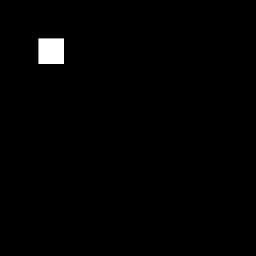
\includegraphics[width=0.3\textwidth]{benchmark-video/frame-00000.png} &
    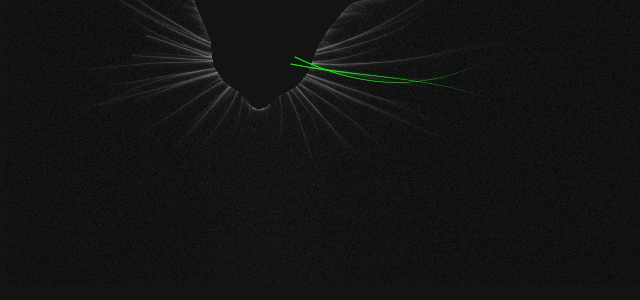
\includegraphics[width=0.3\textwidth]{benchmark-video/frame-00010.png} &
    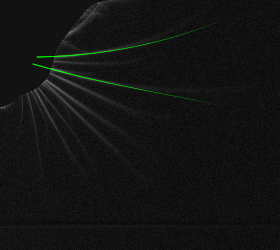
\includegraphics[width=0.3\textwidth]{benchmark-video/frame-00020.png}\\
    Frame 0 & Frame 10 & Frame 20\\
    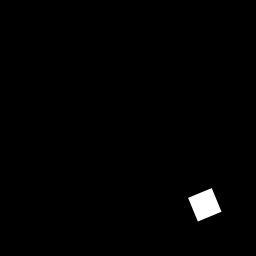
\includegraphics[width=0.3\textwidth]{benchmark-video/frame-00030.png} &
    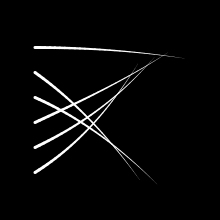
\includegraphics[width=0.3\textwidth]{benchmark-video/frame-00040.png} &
    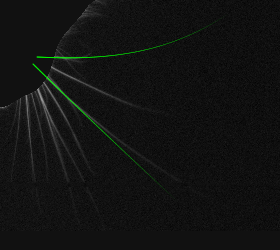
\includegraphics[width=0.3\textwidth]{benchmark-video/frame-00050.png}\\
    Frame 30 & Frame 40 & Frame 50
  \end{tabular}
  \caption{Sample frames from the testing video.}
  \label{fig:benchmark-video}
\end{figure}  


\subsection{Evaluated parameters}
The following parameters were evaluated:

\begin{description}
\item[n] Number of particles
\item[p] In which $\Lp$ space to compute $\Lpnorm{\tf - x_{t-1}}$ in
  the prediction step
\item[a] The exponent for the weights in the prediction step, $w =
  \left(\Lpnorm{\tf - x_{t-1}}\right)^{-a}$
\item[$\sigma$] Standard deviation modifier for the offset in the
  prediction step. Standard deviations for the $\omega^3, \omega^2$
  and $\omega$ terms are $0.1\sigma\sigma_3, 0.1\sigma\sigma_2$ and
  $0.1\sigma\sigma_1$, respectively.\footnote{See section
    \ref{sec:test-data} for the $\sigma_i$ values.}
\item[g] The exponent for the importance in the filtering step
\end{description}

This yields the evaluation tensor $\Phi_{n,p,a,\sigma,g}$.

TODO (check the comments here)
%TODO define phi:img->img
%TODO define \phi(R(x))*\phi(I) as <x,I>_\phi

The measures that will be used as fitness of the parameters:
    \begin{description}
        \item[$\int{||\epsilon(t)||_{L^p}}dt$]
            integrating over time the the difference
            with the ground truth (do this for L{1:10} and see if it correlates with
            the p choosed (to see how much it deviates from the ground truth)
        \item[$\int{\sum{\phi{R(x_t)}\phi{I_t}} }dt$] 
            integrating over time the response
            for the choosed hypothesis (to see how the different image transformation
            affects the results, that is if it only follows what it thinks is best
            (phi))
        \item[Subjective] 4 image samples
    \end{description}
And all this are done for all 4 benchmark videos.


"There are many metrics by which a model may be assessed." - Encyclopedia


The fitness test was runned on different machines but this wont effect the
result since we initially wont consider the running time.

The runtime for the algorithm is handled separately on one machine setup <...>



Tillvägagångsätt:

1. Since we have prior knowledge about the effect off varying the parameters n,N
they will firstly be set to a sufficently large value.
2. A partion of the test-matrix will then be evaluated by ... parameter group 
